\documentclass{article}
\usepackage{amsmath,enumitem,fullpage,graphicx,listings,float,sidecap,setspace,xcolor,wrapfig,booktabs,multirow,subcaption,array,minted,svg,hyperref,xepersian,bidi}

\newcolumntype{C}[1]{>{\centering\arraybackslash}m{#1}}
\definecolor{lg}{HTML}{F4F3F3}
\setlength{\fboxsep}{10pt}
\usemintedstyle{borland}
\hypersetup{
   colorlinks=true,
   linkcolor=blue, % color of internal links
   citecolor=green, % color of links to bibliography
   filecolor=magenta, % color of file links
  urlcolor=cyan % color of external links
}
\setlatintextfont{Vazirmatn}
\settextfont{Vazirmatn}
\begin{document}

\begin{titlepage}
  \centering
  
\includegraphics[width=0.5\textwidth]{iust}\par\vspace{1cm}
  {\scshape\LARGE دانشکده مهندسی کامپیوتر \par}
  \vspace{1cm}
  {\huge\bfseries پروژه درس  \par}
  \vspace{1cm}
  {\Large درس شبکه‌های تلفن همراه \par}
  \vspace{1cm}
  {\large محمد اصولیان، نوید ابراهیمی و سینا علی‌نژاد \par}
  \vspace{5cm}
  {\large نیم سال دوم \par}
  {\large سال تحصیلی ۱۴۰۲-۱۴۰۳ \par}
\end{titlepage}
\newpage
\doublespacing
\section*{مقدمه}  
در پروژه باریم، قرار است یک کلاینت و یک سرور داشته باشیم. برنامه‌ای که بر روی کلاینت قرار دارد، باید همواره به وضعیت سلول خدمتگزار گوش کند و توان دریافتی از آن را بدست آورد. اگر مقدار توان دریافتی از یک حدی کاهش پیدا کرد، پیامی را برای سرور ارسال کند. این پیام باید حاوی اطلاعاتی از سلول خدمتگزار مثل منطقه مکانی(LAC)، تکنولوژی سلول، شناسه سلول و برخی موارد دیگر باشد. 

\section*{ساختار کلی پروژه}
عمده‌ی کد پروژه در سمت کلاینت است، زیرا هم باید اطلاعات سلول خدمتگزار را بخواند و هم باید ارسال پیام انجام دهد. کد پروژه از دو سرویس اندروید تشکیل شده است. یکی همان سرویس اصلی یا main است که در درون آن با زدن دکمه Start یک سرویس دیگر که SignalMonitoring است شروع میشود. این یک سرویس forground است، به این معنا که سیستم نمیتواند به دلایل مختلف مثل کمبود حافظه این سرویس را قطع کند زیرا ارزش آن از سرویس‌های background بیشتر است. هنگامی که کاربر روی دکمه شروع میزند، سرویس SingalMonitoring شروع میشود. درون این سرویس یک Listener تعریف میشود. کار این Listener این است که حواسش به تغییرات قدرت سیگنال باشد و هنگامی که این مقدار تغیر کرد، اطلاعات جدید را از سلول جمع بکند. پس از جمع‌آوری اطلاعات، مقادیر notification نمایشی را تغییر می‌دهد و سپس بررسی میکند که آیا مقدار توان دریافتی از یک حدی کمتر شده است یا خیر. اگر کمتر شده بود، اطلاعات جمع‌آوری شده را در قالب یک پیام برای سرور ارسال می‌کند.  
\singlespacing

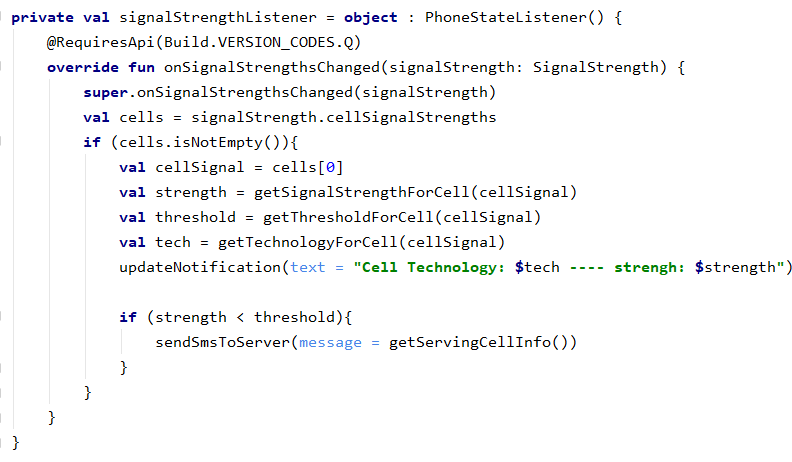
\includegraphics[width=1\textwidth]{listen.png}\par\vspace{1cm}

همچنین در سمت سرور، با اجرای برنامه و درخواست دسترسی‌ها، سرور شروع به شنیدن پیامک ها میکند. در صورتی که پیامک دریافتی در قالب پروتکل مشخص شده نباشد، سرور پاسخی به آن نمیدهد. در صورتی که رمز هش شده درست نباشد، سرور پیام اشتباه بودن رمز را میفرستد و در صورتی که رمز هش شده صحیح باشد، سرور پیام دریافت گزارش را میفرستد
\singlespacing

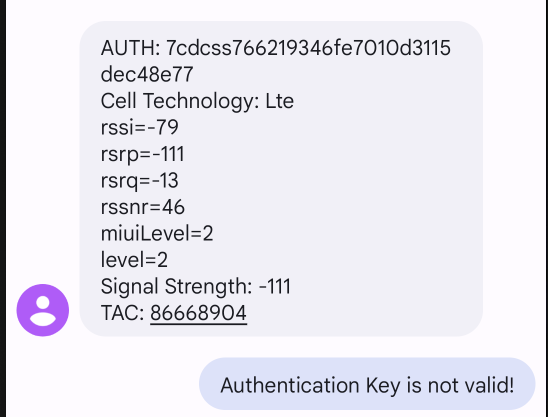
\includegraphics[width=0.5\textwidth]{unauthorized.png}\par\vspace{1cm}
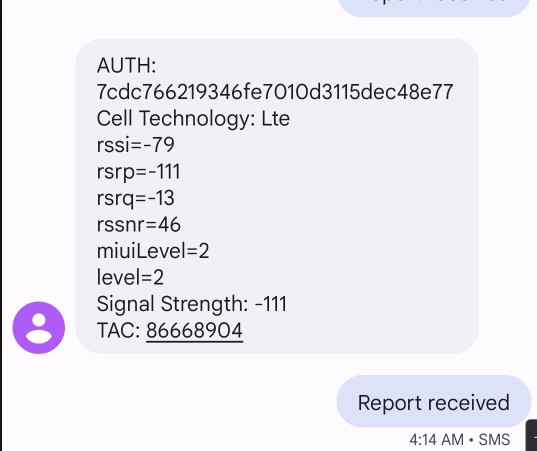
\includegraphics[width=0.5\textwidth]{report.png}\par\vspace{1cm}

در برنامه سرور قابلیت مشاهده و ذخیره سازی لاگ ها هم فراهم شده. کاربرمیتواند وضعیت درخواست هایی که به سرور میشود را مشاهده و در صورت لازم لاگ ها را پاک کند.

\singlespacing
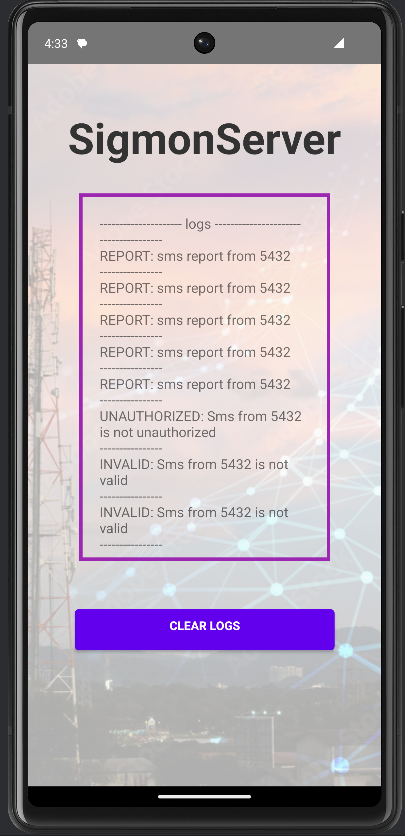
\includegraphics[width=0.5\textwidth]{logs.png}\par\vspace{1cm}



\section*{راهنمای نرم‌افزار}
برای بخش کلاینت یک رابط کاربری ساده نیز زده شد. عکس زیر صفحه اصلی برنامه کلاینت را نشان می‌دهد.
\singlespacing

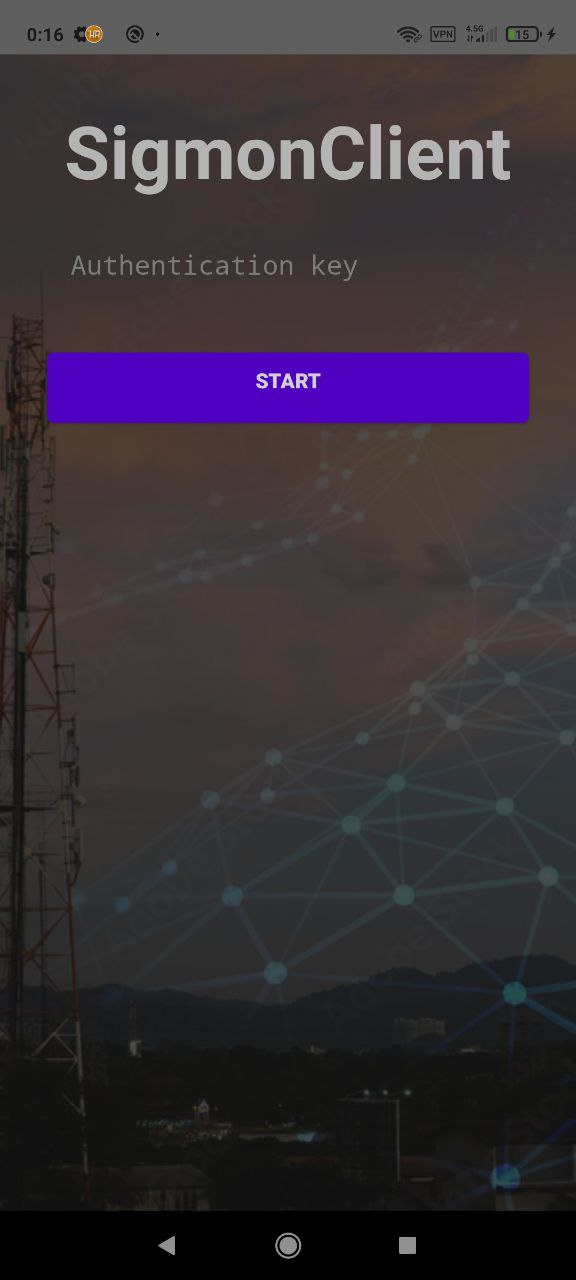
\includegraphics[width=0.3\textwidth]{main.jpg}\par\vspace{1cm}
پس از ورود به برنامه، باید اجازه‌های لازم را برای ارسال و دریافت پیام و همچنین گرفتن اطلاعات سلول و location بدهید.
\singlespacing

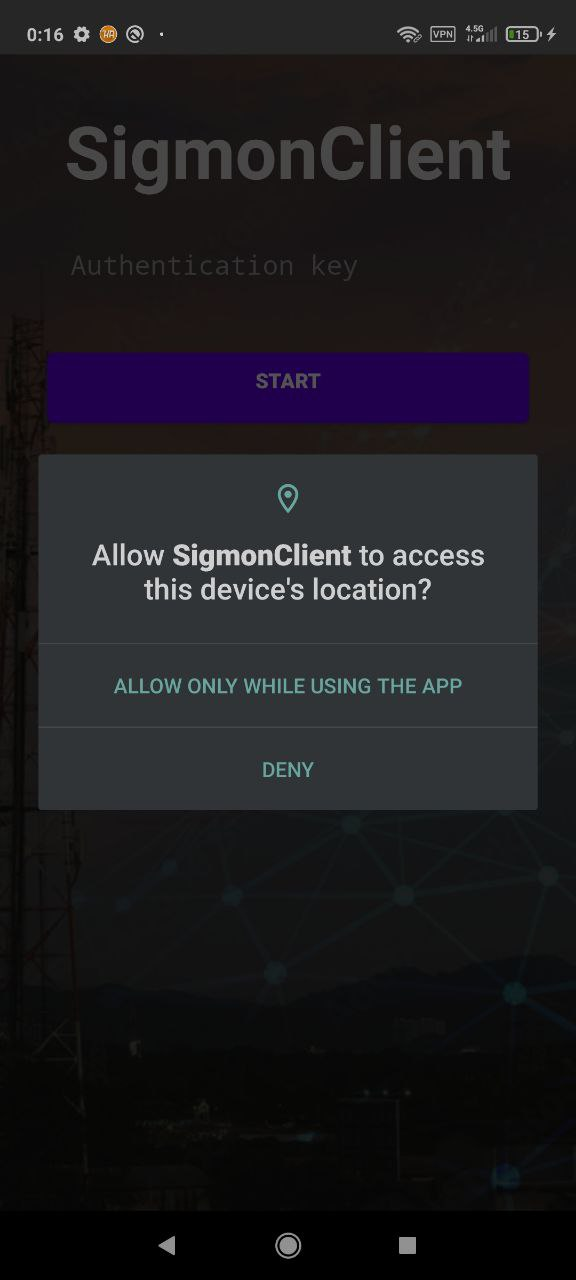
\includegraphics[width=0.25\textwidth]{p1.jpg}\par\vspace{1cm}
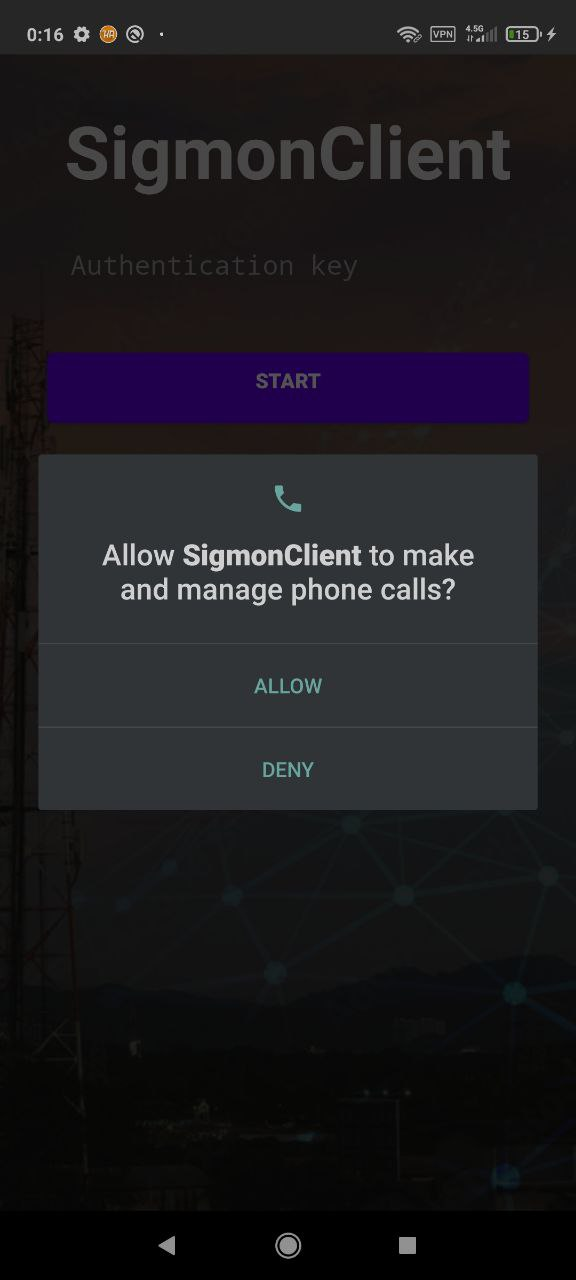
\includegraphics[width=0.25\textwidth]{p2.jpg}\par\vspace{1cm}
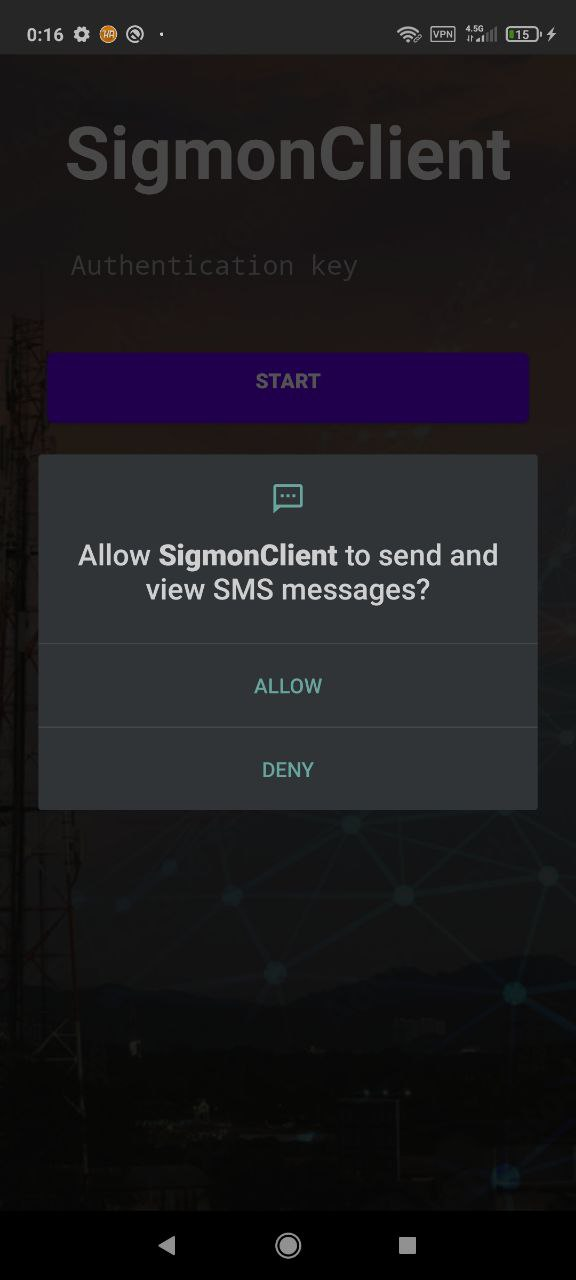
\includegraphics[width=0.3\textwidth]{p3.jpg}\par\vspace{1cm}

ابتدا کاربر باید عملیات register را انجام دهد. پس از آن، سرور یک رمز را به صورت hash شده به کاربر پیامک می‌کند و کاربر می‌تواند از آن برای شروع برنامه استفاده کند. تصویر زیر وارد کردن پسورد را در برنامه نشان می‌دهد.
\singlespacing

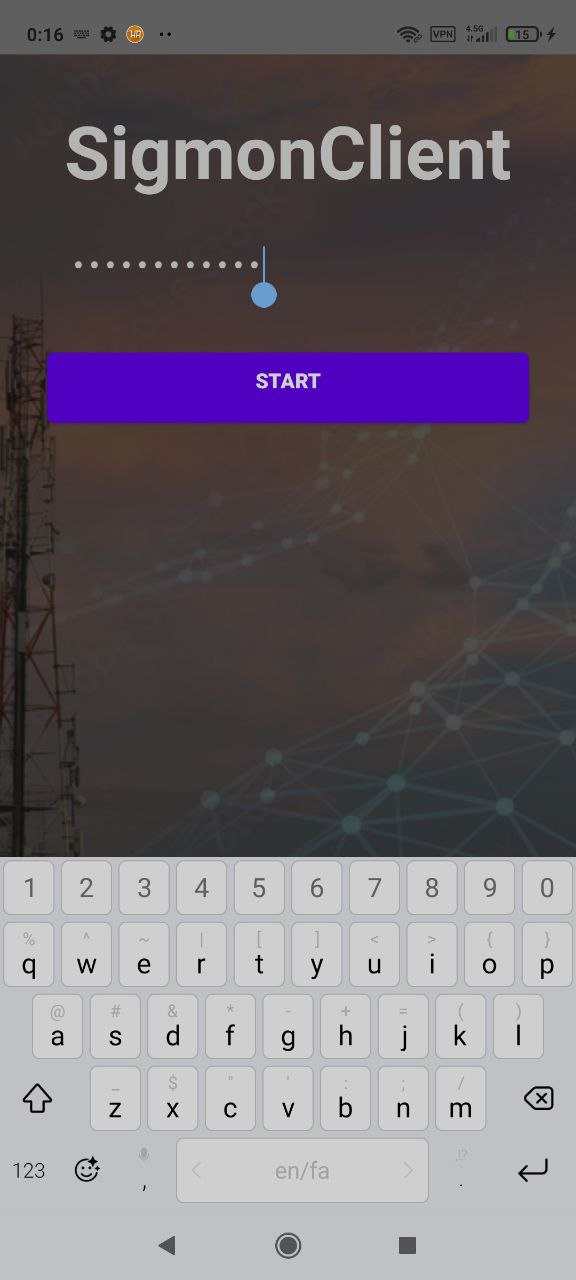
\includegraphics[width=0.3\textwidth]{pass.jpg}\par\vspace{1cm}
پس از زدن دکمه Start نوشته‌ی روی دکمه به Stop تغییر می‌کند و یک پیام به صورت toast در پایین صفحه شروع فرایند را اعلام می‌کند.
\singlespacing

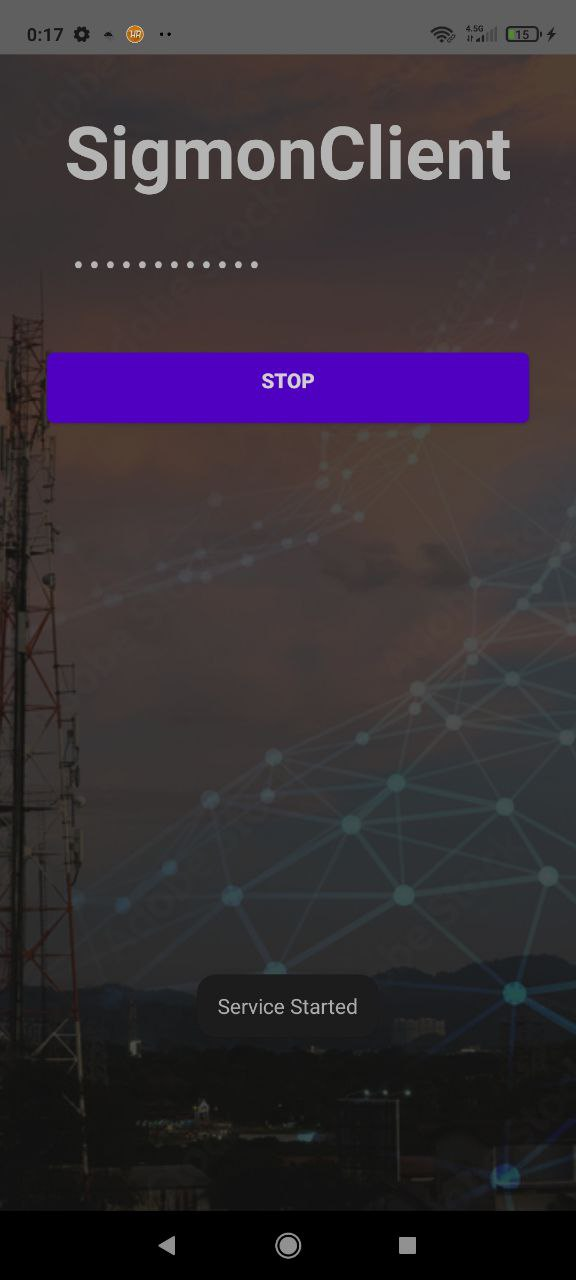
\includegraphics[width=0.3\textwidth]{button_change.jpg}\par\vspace{1cm}
در این حالت وضعیت شبکه، یعنی تکنولوژی سلول و توان دریافتی از آن به صورت یک notification و به صورت live نمایش داده می‌شود.
\singlespacing

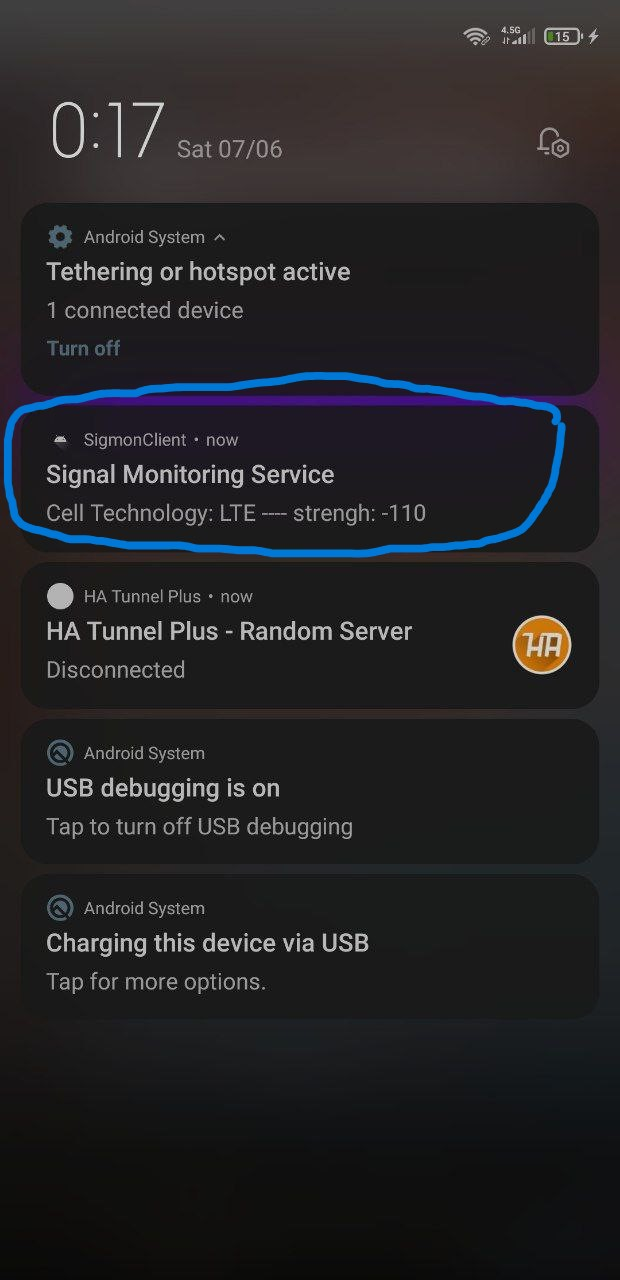
\includegraphics[width=0.3\textwidth]{notif.jpg}\par\vspace{1cm}
همانطور که از عکس مشخص است، تکنولوژی سلول خدمتگزار LTE یا همان 4g است. همچین توان سیگنال دریافتی برابر با dbm 110- است.  
اگر این توان دریافتی از 100- کمتر شود. پیامی را به مانند زیر برای سرور ارسال میکند.
\singlespacing

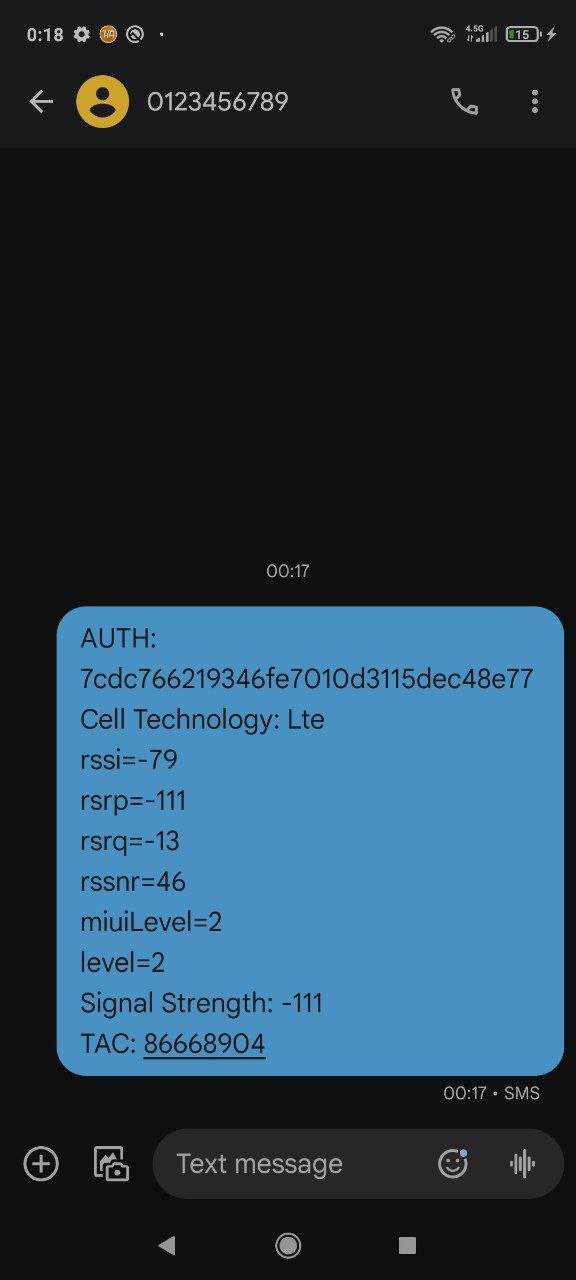
\includegraphics[width=0.4\textwidth]{message.jpg}\par\vspace{1cm}
همانطور که مشخص است، این اطلاعات شامل Key Authentication به صورت hash شده با الگوریتم md5 است. همچنین تکنولوژی سلول و قدرت سیگنال و مواردی که خاص نسل چهارم میباشند مثل TAC و rsrp و rsrq .
در نهایت با زدن دکمه Stop این فرایند متوقف میشود.
\singlespacing

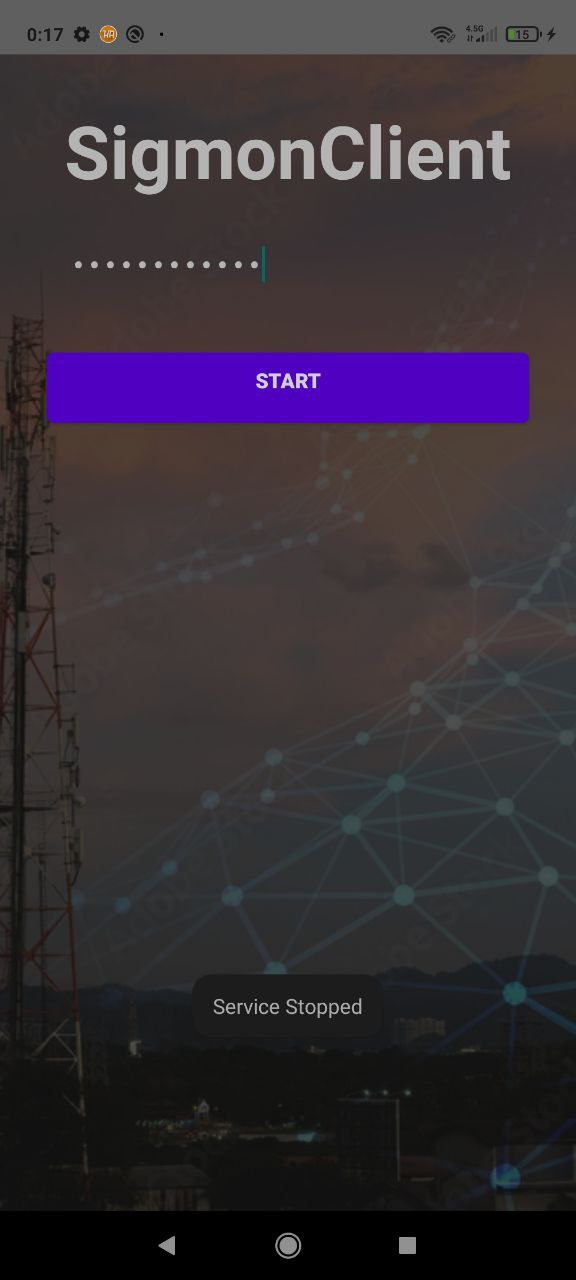
\includegraphics[width=0.3\textwidth]{stop.jpg}\par\vspace{1cm}





\setstretch{1.5}

\end{document}